%%%%%%%%%%%%%%%%%%%%%%%%%%%%%%%%%%%%%%%%%%%%%%%%%%%%%%%%%%%%%%%%%%%%%%%%%%%%%%%%%%%%%%%%%%%%%%%%%
%
% TeX file astrometry-basics-and-interpretation.tex
% Uses: beamer.cls
% Last Updated:  2019.05.03
% First Created: 2019.04.24
%
% Title: Astrometry basics and interpretation of astrometric data
%
% Description: Spitzer Lectures series 2019, Princeton University, May 2019
%
%%%%%%%%%%%%%%%%%%%%%%%%%%%%%%%%%%%%%%%%%%%%%%%%%%%%%%%%%%%%%%%%%%%%%%%%%%%%%%%%%%%%%%%%%%%%%%%%%

\documentclass[smaller, aspectratio=169]{beamer}

\usepackage{times,amsmath,graphicx,marvosym}
\usepackage{tikz}
\usepackage{animate}
\usepackage{colortbl}
\usetikzlibrary{arrows.meta,shapes,calc,shadows,backgrounds}
\usetheme{lightbare169}

\hypersetup{pdftitle={Astrometry basics and interpretation of astrometric data},
pdfsubject={Spitzer Lectures series 2019, Princeton University, May 2019},
pdfauthor={Anthony Brown}, colorlinks=true, linkbordercolor={1 0 0}}

\tikzstyle{flow}=[-{Stealth[round]}, thick, shorten >=3pt, shorten <=3pt]
\tikzstyle{flowboth}=[{Stealth[round]}-{Stealth[round]}, thick, shorten >=3pt, shorten <=3pt]
\tikzstyle{astromvec}=[-{Stealth[round]}, line width=1.5pt, shorten >=3pt, shorten <=3pt]
\tikzstyle{astromvecthin}=[-{Stealth[round]}, line width=0.75pt, shorten >=3pt, shorten <=3pt, color=gray]

\setbeamercovered{invisible}

\graphicspath{ {./Images/} {/home/brown/Gaia/Presentation/Images/} }

\newcommand\gdrone{Gaia~DR1}
\newcommand\gdrtwo{Gaia~DR2}
\newcommand\hip{Hipparcos}
\newcommand\tyctwo{Tycho-2}
\newcommand\tyc{Tycho}
\input{/home/brown/Gaia/Presentation/GaiaDR2OverviewSlides/dr2stats}

\title[Spitzer Lectures May 2019]{Astrometry basics and interpretation of astrometric data}
\author{Anthony Brown}
\institute{Leiden Observatory, Leiden University\\\texttt{brown@strw.leidenuniv.nl}}

\begin{document}
\logos{
}

%\begin{frame}
%  \titlepage
%\end{frame}

\setbeamercolor{background canvas}{bg=black}
\begin{emptyframe}{Title page}
  \hglue-0.57truecm
  \begin{tikzpicture}
    \node (fig) at (current page)
    {\includegraphics[width=15.9cm]{GaiaSky/GaiaDR2/ESA-PR/Gaia_s_sky_in_colour.jpg}};
      \node at ($(fig.south east)+(-0.3,0)$) [anchor=north east, font=\sf\tiny, color=white] {ESA/Gaia/DPAC};
      \node at ($(fig.south west)+(0.5,2.5)$) [anchor=south west, rotate=-45]
      {\includegraphics[height=1.8cm]{Promotion/ArtistsImpression2013.png}};
      \node (title) at ($(current page.north)+(0,-1.0)$) [anchor=north, text width=\textwidth, font=\Huge, text badly centered] {
        \structure{\color{GaiaRed}\inserttitle}
      };
      \node (author) at ($(title.south)+(0,-0.5)$) [anchor=north, text width=\textwidth, font=\Large,
      text badly centered, color=white] {\insertauthor};
      \node (institute) at (author.south) [anchor=north, text width=\textwidth, font=\large, text
      badly centered, color=white] {\insertinstitute};
  \end{tikzpicture}
\end{emptyframe}
\setbeamercolor{background canvas}{bg=white}
%
%%%%%%%%%%%%%%%%%%%%%%%%%%%%%%%%%%%%%%%%%%%%%%%%%%%%%%%%%%%%%%%%%%%%%%%%%%%%%
%
\begin{agaframe}{Scope of this lecture}
  \begin{itemize}
    \item Astrometry developed through vector formulation
    \item Aimed at use and interpretation of modern astrometric catalogue data
    \item Topics not treated
      \begin{itemize}
        \item astrometric measurements and data processing
        \item earth orientation (nutation, precession, etc)
        \item relativistic light deflection
        \item aberration
        \item details of coordinate systems and coordinate transformations
        \item time scales
      \end{itemize}
  \end{itemize}

  \bigskip
  \underbar{Some references}
  \begin{itemize}
    \itemd
      \href{http://gea.esac.esa.int/archive/documentation/GDR2/Data_processing/chap_cu3ast/sec_cu3ast_intro/}{Gaia
      online documentation, chapter 3, section 3.1, 3.3.3}
    \itemd {\em A Practical Relativistic Model for Microarcsecond Astrometry in Space}:
      \href{http://dx.doi.org/10.1086/367593}{Klioner, 2003, AJ 125, p.~1580}
    \itemd {\em The astrometric core solution for the Gaia mission. Overview of models, algorithms,
      and software implementation}: \href{https://doi.org/10.1051/0004-6361/201117905}{Lindegren et
      al., 2012, A\&A 538, A78}
    \itemd {\em Astrometry for Astrophysics}: Methods, Models, and Applications, 2013, ed.~W.F.~van Altena,
      Cambridge University Press (chapters 4, 5, 7)
  \end{itemize}
\end{agaframe}
%
%%%%%%%%%%%%%%%%%%%%%%%%%%%%%%%%%%%%%%%%%%%%%%%%%%%%%%%%%%%%%%%%%%%%%%%%%%%%%
%
\begin{emptyframe}{Astrometry Basics}
  \begin{center}
    \textcolor{GaiaRed}{\Huge Astrometry Basics}
  \end{center}
\end{emptyframe}
%
%%%%%%%%%%%%%%%%%%%%%%%%%%%%%%%%%%%%%%%%%%%%%%%%%%%%%%%%%%%%%%%%%%%%%%%%%%%%%
%
\begin{agaframe}{Vector notation used here}
  \centering
  \begin{equation}
    \vect{a} = \begin{bmatrix}
      a_x \\ a_y \\ a_z\\
    \end{bmatrix}
    \label{eq:defvect}
  \end{equation}
  $\transposep{\vect{a}}$: transpose of vector \vect{a}
  
  \medskip
  Inner product and cross-product
  \begin{equation}
    \transposep{\vect{a}}\vect{b} = a_xb_x+a_yb_y+a_zb_z
    \quad\text{and}\quad
    \vect{a}\times\vect{b} = \begin{bmatrix}
      a_yb_z-a_zb_y \\
      a_zb_x-a_xb_z \\
      a_xb_y-a_yb_x \\
    \end{bmatrix}
    \label{eq:defdotcross}
  \end{equation}

  \medskip
  normalization: $|\vect{a}| = \sqrt{\transposep{\vect{a}}\vect{a}} = (a_x^2+a_y^2+a_z^2)^{1/2}$

  \begin{equation}
    \langle\vect{a}\rangle = \vect{a}|\vect{a}|^{-1}
  \end{equation}
\end{agaframe}
%
%%%%%%%%%%%%%%%%%%%%%%%%%%%%%%%%%%%%%%%%%%%%%%%%%%%%%%%%%%%%%%%%%%%%%%%%%%%%%
%
\begin{agaframe}{Celestial coordinates and reference systems}
  \begin{tikzpicture}
    \node (icrs) {\includegraphics[height=5.5cm]{Astrometry/icrs-coordinates.pdf}};
    \node at (icrs.east) [anchor=west, text width=9cm, text badly ragged] {
      \begin{itemize}
        \item Celestial positions $(\alpha,\delta)$ of sources $S$ are referred to an idealized
          coordinate system, the International Celestial Reference System (ICRS)
          \begin{itemize}
            \item origin at the solar system barycentre
          \end{itemize}
        \item Kinematically defined with {\em fixed axis directions} with respect to distant matter in the
          universe
          \begin{itemize}
            \item principle plane close to mean equator at J2000.0, with origin close to dynamical
              equinox at J2000.0
            \item there is no precession/nutation of the axes!
            \item i.e., transforming source coordinates to a different epoch only involves the
              proper motion!
          \end{itemize}
        \item Practical realization is the International Celestial Reference Frame (ICRF)
          \begin{itemize}
            \item defined through precise coordinates of extragalactic objects
            \item $\sim4500$ sources for radio frame (ICRF3), $\sim550\,000$ sources for optical frame
              (Gaia-CRF2)
            \item frames aligned through overlapping sources: limited by differences in physical
              origin of radio/optical emission
          \end{itemize}
      \end{itemize}
    };
  \end{tikzpicture}
\end{agaframe}
%
%%%%%%%%%%%%%%%%%%%%%%%%%%%%%%%%%%%%%%%%%%%%%%%%%%%%%%%%%%%%%%%%%%%%%%%%%%%%%
%
\begin{agaframe}{Astrometry: observational process}
  \begin{itemize}
    \item Astrometric measurements consist of repeated measurements of the directions to sources on
      the sky
    \item The celestial directions have to be {\em modelled} to extract the astrometric parameters
      (position, parallax, proper motion, etc) of interest
    \item The modelling includes:
      \begin{itemize}
        \item source model
        \item light propagation model
        \item observer's orbit (for aberration correction, parallax scaling, and solar system
          objects)
        \item observer's orientation (spacecraft attitude for Gaia)
      \end{itemize}
    \item Light propagation and aberration are ignored in the following
    \item Solar system object astrometry is not treated
  \end{itemize}
\end{agaframe}
%
%%%%%%%%%%%%%%%%%%%%%%%%%%%%%%%%%%%%%%%%%%%%%%%%%%%%%%%%%%%%%%%%%%%%%%%%%%%%%
%
\begin{agaframe}{Schematic of Gaia observational process}
  \begin{tikzpicture}
    \node (fig)
    {\includegraphics[height=7cm]{DataProcessing/data-processing-schematic-agis-sacg-crop.pdf}};
    \node at (fig.south east) [anchor=south west, text width=5cm, text badly ragged,
    font=\scriptsize] {
      This is an illustration of the practical challenges of astrometry with Gaia. The details
      behind this schematic not treated in the following slides. Image credits: ESA/Airbus DS.
    };
  \end{tikzpicture}
\end{agaframe}
%
%%%%%%%%%%%%%%%%%%%%%%%%%%%%%%%%%%%%%%%%%%%%%%%%%%%%%%%%%%%%%%%%%%%%%%%%%%%%%
%
\begin{agaframe}{Modelling source positions}
  \begin{tikzpicture}
    \node (bcrs) {\includegraphics[height=5.5cm]{Astrometry/bcrs-source-position.pdf}};
    \node at (bcrs.east) [anchor=west, text width=9cm, text badly ragged] {
      \begin{itemize}
        \item Source directions are modelled in the Barycentric Celestial Reference System (BCRS)
          \begin{itemize}
            \item includes parallax, aberration, and relativistic light deflection for apparent
              directions
            \item BCRS is a system of space-time coordinates for the solar system in the framework
              of General Relativity with a specific metric tensor
            \item aligned with ICRS
            \item associated time scale is Barycentric Coordinate Time (TCB)
          \end{itemize}
      \end{itemize}

      \medskip
      \underbar{Barycentric source coordinates}
      \begin{itemize}
        \itemd Source $S$ at distance $b$ from solar system barycentre ($B$)
        \itemd Barycentric coordinates of $S$: $\vect{b} = b\vect{u}$, with \vect{u} the direction
          from $B$ to $S$
      \end{itemize}
      \begin{equation}
        \vect{u} = \begin{bmatrix} \cos\delta\cos\alpha \\ \cos\delta\sin\alpha \\ \sin\delta
        \end{bmatrix}
      \end{equation}
    };
  \end{tikzpicture}
\end{agaframe}
%
%%%%%%%%%%%%%%%%%%%%%%%%%%%%%%%%%%%%%%%%%%%%%%%%%%%%%%%%%%%%%%%%%%%%%%%%%%%%%
%
\begin{agaframe}{Modelling source motion I}
  \begin{tikzpicture}
    \node (fig) {\includegraphics[width=6cm]{Astrometry/source-motion-and-celestial-sphere.pdf}};
    \node at (fig.east) [anchor=west, text width=9cm, text badly ragged] {
      Standard model for stellar motion:
      \begin{equation}
        \vect{b}(t) = \vect{b}_\mathrm{ep}+(t-t_\mathrm{ep})\vect{v}\,, \quad
        \vect{u}(t) = \langle \vect{b}_\mathrm{ep}+(t-t_\mathrm{ep})\vect{v} \rangle
        \label{eq:sourcemodel}
      \end{equation}

      Proper motion and (astrometric!) radial velocity:
      \begin{equation}
        \vect{\mu}(t) = \frac{d\vect{u}}{dt}\,, \quad v_\mathrm{rad}(t) = \frac{db}{dt}
        \label{eq:pmandvrad}
      \end{equation}
      Note the time dependence of \vect{\mu} and $v_\mathrm{rad}$ $\longrightarrow$ `perspective
      acceleration' for nearby fast moving stars. To good approximation:
      \begin{equation}
        \mu = \frac{v_\mathrm{tan}}{b}\, \quad v_\mathrm{rad} = \transposep{\vect{v}}\vect{u}
        \label{eq:pmvradapprox}
      \end{equation}

      \medskip
      Astrometric and spectroscopic radial velocity are not the same: see
      \href{https://doi.org/10.1051/0004-6361:20030181}{Lindegren \& Dravins (2003)}
    };
  \end{tikzpicture}
\end{agaframe}
%
%%%%%%%%%%%%%%%%%%%%%%%%%%%%%%%%%%%%%%%%%%%%%%%%%%%%%%%%%%%%%%%%%%%%%%%%%%%%%
%
\begin{agaframe}{Modelling source motion II}
  \begin{tikzpicture}
    \node (fig) {\includegraphics[width=6cm]{Astrometry/bcrs-normaltriad.pdf}};
    \node at (fig.east) [anchor=west, text width=9cm, text badly ragged] {
      `Normal triad' $\begin{bmatrix}\vect{p} & \vect{q} & \vect{r}\end{bmatrix}$:
      \begin{equation}
        \vect{r} = \vect{u}_\mathrm{ep}\,,\quad \vect{p}=\langle\vect{z}\times\vect{r}\rangle\,, \quad
        \vect{q}=\vect{r}\times\vect{p}
        \label{eq:pqrdef}
      \end{equation}
      \begin{equation}
        \begin{bmatrix}\vect{p} & \vect{q} & \vect{r}\end{bmatrix} = 
        \begin{bmatrix}
          -\sin\alpha & -\sin\delta\cos\alpha & \cos\delta\cos\alpha \\
          \cos\alpha & -\sin\delta\sin\alpha & \cos\delta\sin\alpha \\
          0 & \cos\delta & \sin\delta
        \end{bmatrix}
        \label{eq:pqrcomps}
      \end{equation}

      \begin{equation}
        \frac{\partial\vect{r}}{\partial \alpha} = \vect{p}\cos\delta\,, \quad
        \frac{\partial\vect{r}}{\partial \delta} = \vect{q} \,,\quad
        d\vect{r} = \vect{p}d\alpha\cos\delta+\vect{q}d\delta
        \label{eq:rdifferentials}
      \end{equation}
      \begin{equation}
        \mu_\alpha = \frac{d\alpha}{dt}\,,\quad \mu_{\alpha*} = \frac{d\alpha}{dt}\cos\delta\,,\quad \mu_\delta = \frac{d\delta}{dt}
        \label{eq:propermotiondef}
      \end{equation}

      {\mura} and {\mudec} can be seen as projections of $d\vect{r}/dt$ on \vect{p} and \vect{q}.
      In general $\vect{u}(t)$ is different from \vect{r}, so express \vect{\mu} with respect to
      fixed triad:
      \begin{equation}
        \vect{\mu} = \frac{d\vect{u}}{dt} = \vect{p}\mura + \vect{q}\mudec
        \label{eq:propermotionpqr}
      \end{equation}
    };
  \end{tikzpicture}
\end{agaframe}
%
%%%%%%%%%%%%%%%%%%%%%%%%%%%%%%%%%%%%%%%%%%%%%%%%%%%%%%%%%%%%%%%%%%%%%%%%%%%%%
%
\begin{agaframe}{Modelling source motion III}
  \begin{tikzpicture}
    \node (fig) {\includegraphics[width=6cm]{Astrometry/bcrs-normaltriad.pdf}};
    \node at (fig.east) [anchor=west, text width=8cm, text badly ragged, xshift=0.5cm] {
      Source velocity in terms of $\begin{bmatrix}\vect{p} & \vect{q} & \vect{r}\end{bmatrix}$:
      \begin{equation}
        \vect{v} = \vect{v}_\mathrm{tan}+\vect{r}v_\mathrm{rad} = \vect{\mu}A_v b +
        \vect{r}v_\mathrm{rad}\nonumber
      \end{equation}
      \begin{equation}
        \vect{v} = \vect{p}\mura A_v/\varpi + \vect{q}\mudec A_v/\varpi + \vect{r}v_\mathrm{rad}\,,
        \label{eq:velpqr}
      \end{equation}

      \smallskip
      with $A_v = 4.74047\dots$~km~yr~s$^{-1}$ and $\varpi=1/b$.
    };
    \node at (fig.south east) [anchor=north west, text width=10.5cm, text badly ragged, xshift=-3cm,
    yshift=1cm] {
      \hfill Eq.~\eqref{eq:velpqr} is a rotation:
      \begin{equation}
        \vect{v} = \begin{bmatrix} v_x\\ v_y\\ v_z\end{bmatrix} =
        \begin{bmatrix}
          -\sin\alpha & -\sin\delta\cos\alpha & \cos\delta\cos\alpha \\
          \cos\alpha & -\sin\delta\sin\alpha & \cos\delta\sin\alpha \\
          0 & \cos\delta & \sin\delta
        \end{bmatrix}
        \begin{bmatrix}
          \mura A_v/\varpi \\ \mudec A_v/\varpi \\ v_\mathrm{rad}
        \end{bmatrix}
        \label{eq:velpqrasrot}
      \end{equation}
    };
  \end{tikzpicture}
\end{agaframe}
%
%%%%%%%%%%%%%%%%%%%%%%%%%%%%%%%%%%%%%%%%%%%%%%%%%%%%%%%%%%%%%%%%%%%%%%%%%%%%%
%
\begin{agaframe}[1-2]{Source motion including parallax}
  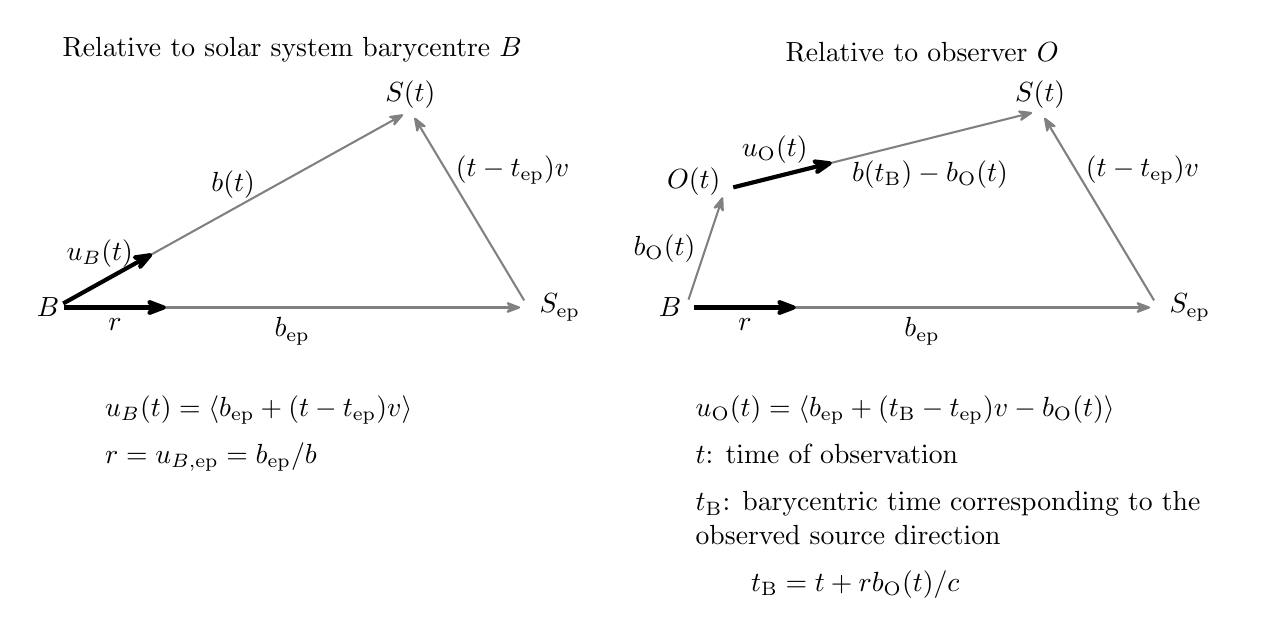
\begin{tikzpicture}
    \coordinate (bary) at (0,0);
    \coordinate (sourceA) at ($(bary)+(6,0)$);
    \coordinate (sourceB) at ($(sourceA)+(-1.5,2.5)$);

    \draw[astromvecthin] (bary) -- node[below, color=black] {$\vect{b}_\mathrm{ep}$} (sourceA);
    \draw[astromvecthin] (bary) -- node[above, color=black] {$\vect{b}(t)$} (sourceB);
    \draw[astromvecthin] (sourceA) -- node[right, color=black, pos=0.7] {$(t-t_\mathrm{ep})\vect{v}$} (sourceB);
    \draw[astromvec] (bary) -- node [below] {$\vect{r}$} ($(bary)!1.5cm!(sourceA)$);
    \draw[astromvec] (bary) -- node [above, xshift=-0.1cm] {$\vect{u}_B(t)$} ($(bary)!1.5cm!(sourceB)$);

    \node at ($(bary)+(-0.1,0)$) {$B$};
    \node at ($(sourceA)+(0.4,0)$) {$S_\mathrm{ep}$};
    \node at ($(sourceB)+(0,0.2)$) {$S(t)$};

    \node at ($(bary)!0.5!(sourceA)+(0,3)$) [anchor=south] {Relative to solar system barycentre $B$};

    \node at ($(bary)+(0.5,-1)$) [anchor=north west, text width=7cm, text badly ragged] {
      $\vect{u}_B(t) = \langle\vect{b}_\mathrm{ep}+(t-t_\mathrm{ep})\vect{v}\rangle$\\[5pt]
      $\vect{r} = \vect{u}_{B,\mathrm{ep}} = \vect{b}_\mathrm{ep}/b$
    };

    \uncover<2->{
      \coordinate (baryB) at ($(bary)+(8,0)$);
      \coordinate (observer) at ($(baryB)+(0.5,1.5)$);
      \coordinate (sourceBA) at ($(baryB)+(6,0)$);
      \coordinate (sourceBB) at ($(sourceBA)+(-1.5,2.5)$);

      \draw[astromvecthin] (baryB) -- node[below, color=black] {$\vect{b}_\mathrm{ep}$} (sourceBA);
      \draw[astromvecthin] (baryB) -- node[left, color=black] {$\vect{b}_\mathrm{O}(t)$} (observer);
      \draw[astromvecthin] (observer) -- node[below, xshift=0.6cm, yshift=0.0cm, color=black]
      {$\vect{b}(t_\mathrm{B})-\vect{b}_\mathrm{O}(t)$} (sourceBB);
      \draw[astromvecthin] (sourceBA) -- node[right, color=black, pos=0.7] {$(t-t_\mathrm{ep})\vect{v}$} (sourceBB);
      \draw[astromvec] (baryB) -- node [below] {$\vect{r}$} ($(baryB)!1.5cm!(sourceBA)$);
      \draw[astromvec] (observer) -- node [above, xshift=-0.1cm] {$\vect{u}_\mathrm{O}(t)$}
      ($(observer)!1.5cm!(sourceBB)$);

      \node at ($(baryB)+(-0.2,0)$) {$B$};
      \node at ($(observer)+(-0.4,0.1)$) {$O(t)$};
      \node at ($(sourceBA)+(0.4,0)$) {$S_\mathrm{ep}$};
      \node at ($(sourceBB)+(0,0.2)$) {$S(t)$};

      \node at ($(baryB)!0.5!(sourceBA)+(0,3)$) [anchor=south] {Relative to observer $O$};

      \node at ($(baryB)+(0.0,-1)$) [anchor=north west, text width=7cm, text badly ragged] {
        $\vect{u}_\mathrm{O}(t) = \langle\vect{b}_\mathrm{ep} + (t_\mathrm{B}-t_\mathrm{ep})\vect{v}
        - \vect{b}_\mathrm{O}(t)\rangle$\\[5pt]
        $t$: time of observation\\[5pt]
        $t_\mathrm{B}$: barycentric time corresponding to the observed source direction\\[5pt]
        \hskip2em $t_\mathrm{B} = t + \transposep{\vect{r}}\vect{b}_\mathrm{O}(t)/c$
      };
    }
  \end{tikzpicture}
\end{agaframe}
%
%%%%%%%%%%%%%%%%%%%%%%%%%%%%%%%%%%%%%%%%%%%%%%%%%%%%%%%%%%%%%%%%%%%%%%%%%%%%%
%
\begin{agaframe}{Astrometric source model}
  \underbar{Source model in terms of astrometric parameters}\\[3pt]
  Only coordinate directions are modelled here; light bending and aberration not included
  \begin{gather}
    \vect{u}_\mathrm{O}(t) = \langle b \times [\vect{u}_{B,\mathrm{ep}}+(t_\mathrm{B}-t_\mathrm{ep})\vect{v}/b -
    \vect{b}_\mathrm{O}(t)/b]\rangle\nonumber \\[5pt]
    \vect{u}_\mathrm{O}(t) = \langle \vect{r}+(t_\mathrm{B}-t_\mathrm{ep})
    (\vect{p}\mura + \vect{q}\mudec  + \vect{r}\mu_r) - \vect{b}_\mathrm{O}(t)\varpi/A_\mathrm{u} \rangle
    \label{eq:sourcemodelA}
  \end{gather}
  $\mu_r = v_\mathrm{rad}\varpi/A_v$ is the `radial proper motion' which accounts for perspective
  acceleration. All angles here in radians, distances in AU, time in Julian years.

  \bigskip
  \underbar{Simplified astrometric equations}\\[3pt]
  Assume we have access directly to measurements $(\Delta\alpha(t),\Delta\delta(t))$ with respect to
  some known reference position $(\alpha(t_\mathrm{ep}),\delta(t_\mathrm{ep}))$
  \begin{equation}
    \begin{aligned}
      \Delta\alpha\!\ast\!(t) = \Delta\alpha(t)\cos\delta(t) & = \vect{p}'\vect{u}_\mathrm{O}(t) \approx (t_\mathrm{B}-t_\mathrm{ep})\mu_{\alpha*} -
      \varpi\boldsymbol{p}'\boldsymbol{b}_\mathrm{O}(t)/A_\mathrm{u}\\[5pt]
      \Delta\delta(t) & = \vect{q}'\vect{u}_\mathrm{O}(t) \approx (t_\mathrm{B}-t_\mathrm{ep})\mu_{\delta} -
      \varpi\boldsymbol{q}'\boldsymbol{b}_\mathrm{O}(t)/A_\mathrm{u}
    \end{aligned}
    \label{eq:simplifiedeqs}
  \end{equation}
\end{agaframe}
%
%%%%%%%%%%%%%%%%%%%%%%%%%%%%%%%%%%%%%%%%%%%%%%%%%%%%%%%%%%%%%%%%%%%%%%%%%%%%%
%
\begin{emptyframe}{Use of astrometric data}
  \begin{center}
    \textcolor{GaiaRed}{\Huge Use and interpretation of astrometric data}
  \end{center}
\end{emptyframe}
%
%%%%%%%%%%%%%%%%%%%%%%%%%%%%%%%%%%%%%%%%%%%%%%%%%%%%%%%%%%%%%%%%%%%%%%%%%%%%%
%
\begin{agaframe}{Remarks}
  The following material was developed with the analysis of Gaia catalogue data in mind. However,
  most of the considerations are not exclusive to Gaia catalogue data but apply to data analysis in
  general.

  \bigskip
  The presentation slides largely follow the paper by Luri et~al. (2018), `Gaia Data Release 2:
  Using Gaia Parallaxes', \url{https://doi.org/10.1051/0004-6361/201832964}.

  \bigskip
  Corresponding Python/R notebooks at:
  \url{https://github.com/agabrown/astrometry-inference-tutorials}
\end{agaframe}
%
%
\section[Uncertainties]{Uncertainties in the Gaia catalogue(s)}
%
%%%%%%%%%%%%%%%%%%%%%%%%%%%%%%%%%%%%%%%%%%%%%%%%%%%%%%%%%%%%%%%%%%%%%%%%%%%%%
%
\begin{agaframe}{Gaia DR2 astrometry: uncertainties and systematic errors}
  \begin{tikzpicture}
    \node (fig) {\includegraphics[height=5cm]{UseOfGaiaAstrometry/qso-parallaxes-DR2-hist.pdf}};
    \node at ($(fig.south)+(-0.5,-1)$) [anchor=east, font=\tiny] {Images:
    \href{https://doi.org/10.1051/0004-6361/201832727}{Lindegren et al. (2018)}};
    \node at ($(fig.north)+(0.2,-0.2)$) [anchor=south, font=\scriptsize] {QSO parallaxes};
    \node at ($(fig.north east)+(0,0.8)$) [anchor=north west, text width=8.5cm, text badly ragged] {
      \begin{itemize}
        \item Uncertainties are nearly Gaussian
          \begin{itemize}
            \item NOTE: uncertainties on the astrometric parameters are correlated
          \end{itemize}
        \item Dependencies on celestial position, magnitude, colour
        \item Systematic errors are present
          \begin{itemize}
            \item non-zero mean of Gaussian uncertainty
            \item dependencies on celestial position, magnitude, colour
            \item spatially correlated
          \end{itemize}
      \end{itemize}
    };
    \node (lmc) at ($(fig.south east)+(3.5,2.3)$) [anchor=north west]
    {\includegraphics[height=4.0cm]{GaiaDR2/Contents/lmcPlxMapLabelled.pdf}};
    \node at ($(lmc.south west)+(0,1)$) [anchor=south east, text width=3cm, text badly ragged, font=\scriptsize] {Median
    parallax LMC region};
  \end{tikzpicture}
\end{agaframe}
%
%%%%%%%%%%%%%%%%%%%%%%%%%%%%%%%%%%%%%%%%%%%%%%%%%%%%%%%%%%%%%%%%%%%%%%%%%%%%%
%
\begin{agaframe}[1-5]{Correlated uncertainties}
  \only<1>{
    Covariance matrix for a measured $k$-dimensional vector of quantities \vect{x}:
    \begin{equation*}
      \mat{C}_{ij} = E[(x_i-\mu_i)(x_j-\mu_j)] = \rho_i^j\sigma_i\sigma_j \quad\quad \mu_i=E(x_i) 
    \end{equation*}
    Distribution of \vect{x} around mean \vect{\mu} can be treated as multivariate normal:
    \begin{equation*}
      p(\vect{x}|\vect{\mu},\mat{C}) = {\cal N}_k(\vect{\mu}, \mat{C}) =
      \frac{1}{\sqrt{(2\pi)^k\det(\mat{C})}}
      \exp\left( -\frac{1}{2}(\vect{x}-\vect{\mu})' \mat{C}^{-1} (\vect{x}-\vect{\mu}) \right)
    \end{equation*}
    Transformation:
    \begin{equation*}
      \vect{y} = \vect{f}(\vect{x}) \quad\longrightarrow\quad \mat{C}_{\vect{y}} =
      \mat{J}_f\mat{C}_{\vect{x}}\mat{J}_f^\prime \quad\quad \mat{J}_{ij} = \frac{\partial
      f_i}{\partial x_j}
    \end{equation*}
    Example:
    \begin{equation*}
      \begin{pmatrix} \mu_{l*}\\ \mu_b \end{pmatrix} =
      \begin{pmatrix} 
        c & s \\
        -s & c
      \end{pmatrix}
      \begin{pmatrix} 
        \mu_{\alpha*} \\ \mu_\delta
      \end{pmatrix}
      \quad\quad
      \mat{C}_{lb} = 
      \begin{pmatrix} 
        c & s \\
        -s & c
      \end{pmatrix}
      \begin{pmatrix}
        \sigma_{\mu_{\alpha *}}^2 & \rho_{\mu_{\alpha *}}^{\mu_{\delta}} \sigma_{\mu_{\alpha *}}
        \sigma_{\mu_\delta}\\ 
        \rho_{\mu_{\alpha *}}^{\mu_{\delta}} \sigma_{\mu_{\alpha *}} \sigma_{\mu_\delta}
        & \sigma_{\mu_\delta}^2
      \end{pmatrix}
      \begin{pmatrix} 
        c & -s \\
        s & c
      \end{pmatrix}
    \end{equation*}
    \hskip2cm $c=c(\alpha,\delta)$, $s=s(\alpha,\delta)$
  }
  \only<2>{
    \begin{tikzpicture}
      \node (xy) {\includegraphics[height=3.5cm]{UseOfGaiaAstrometry/CovMatXY.pdf}};
      \node (ab) at (xy.south) [anchor=north]
      {\includegraphics[height=3.5cm]{UseOfGaiaAstrometry/CovMatAB.pdf}};
      \node (text) at (xy.north west) [anchor=north east, text width=10cm, text badly ragged,
      font=\scriptsize]{
        \underbar{Example}\\[5pt]
        Measurements of $x$ and $y$, uncertainties are uncorrelated ($\sigma_{xy}=0$):
        \begin{equation*}
          \vect{\mu}_{xy} = \begin{pmatrix} 1 \\ 2\end{pmatrix} \quad \mat{C}_{xy} =
          \begin{pmatrix}
            \sigma^2_x & \sigma_{xy} \\ \sigma_{xy} & \sigma^2_y
          \end{pmatrix}
          =
          \begin{pmatrix} 0.4 & 0 \\ 0 & 0.1\end{pmatrix}
        \end{equation*}
        \begin{equation*}
          p(x,y) = \frac{1}{0.4\pi} \exp\left( -\frac{1}{2}\left( \frac{(x-1)^2}{0.4} +
          \frac{(y-2)^2}{0.1}\right)\right)
        \end{equation*}
        
        \medskip
        New quantities $a=x+y$, $b=x-y$:
        \begin{equation*}
          \mat{J}=\begin{pmatrix} \partial a/\partial x & \partial a/\partial y \\
          \partial b/\partial x & \partial b/\partial y \end{pmatrix} =
          \begin{pmatrix} 1 & 1 \\ 1 & -1\end{pmatrix}
        \end{equation*}

        \begin{equation*}
          \vect{\mu}_{ab} = \begin{pmatrix} 3 \\ -1\end{pmatrix} \quad 
          \mat{C}_{ab} = \begin{pmatrix}
            \sigma^2_x+\sigma^2_y & \sigma^2_x-\sigma^2_y \\
            \sigma^2_x-\sigma^2_y & \sigma^2_x+\sigma^2_y \\
          \end{pmatrix} = 
          \begin{pmatrix} 0.5 & 0.3 \\ 0.3 & 0.5\end{pmatrix} \quad (\rho=0.6)
        \end{equation*}

        \begin{equation*}
          p(a,b) = \frac{1}{0.8\pi} \exp\left( -\frac{1}{1.28}\left( \frac{(a-3)^2}{0.5} +
          \frac{(b+1)^2}{0.5} - \frac{1.2(a-3)(b+1)}{0.5} \right)\right)
        \end{equation*}
      };
      \draw[flow] ($(text)+(3,0.7)$) -- ($(xy.south west)+(-0.2,1.5)$);
      \draw[flow] ($(text.south east)+(-0.8,0.4)$) -- ($(ab.south west)+(0.2,1.5)$);
    \end{tikzpicture}
  }
  \only<3>{
    \underbar{Simple Python simulation of material on previous slide}
    \begin{columns}
      \begin{column}{0.55\textwidth}
        {\scriptsize
        \begin{semiverbatim}
        import numpy as np

        import matplotlib.pyplot as plt

        from scipy.stats import norm
        

        x = norm.rvs(loc=1, scale=np.sqrt(0.4), size=1000)
        
        y = norm.rvs(loc=2, scale=np.sqrt(0.1), size=1000)
        
        a = x+y
        
        b = x-y
        
        
        plt.plot(x, y, '.', label=r'\$(x,y)\$')
        
        plt.plot(a, b, '+', label=r'\$(a,b)\$')
        
        plt.legend()
        
        plt.show()
        \end{semiverbatim}}
      \end{column}
      \begin{column}{0.45\textwidth}
        \includegraphics[height=5cm]{UseOfGaiaAstrometry/simulated-covmat-transform.png}
      \end{column}
    \end{columns}
  }
  \only<4>{
    Account for covariances in your data analysis when:
    \begin{itemize}
      \item propagating uncertainties on subsets and/or linear combinations of astrometric
        parameters
      \item estimating model parameters: $\chi^2$-fitting, maximum likelihood, Bayesian
        inference, etc
      \item sampling the astrometric uncertainties in some Monte Carlo procedure
        \begin{itemize}
          \item usually better to sample in the astrometric parameters before transforming to, e.g.,
            phase space quantities
        \end{itemize}
    \end{itemize}
  }
  \only<5>{
    \begin{tikzpicture}
      \node (fig) {\includegraphics[height=6cm]{UseOfGaiaAstrometry/hyades_vresiduals.pdf}};
      \node at (fig.south) [anchor=north, text width=6cm, text badly ragged] {Hyades velocity
      residuals suggest shear/rotation in cluster. Is it real?};
      \node at (fig.north east) [anchor=north west, text width=8cm, text badly ragged] {
        \begin{itemize}
          \item Transformation from astrometric parameters to Cartesian positions/velocities will introduce
            correlations in the propagated uncertainties
            \begin{itemize}
              \item even in the absence of correlations in the observables, as speed = proper
                motion/parallax
            \end{itemize}
          \item In this case similar proper motion vectors for the cluster members lead to apparent
            correlations between velocity residuals and positions
            \begin{itemize}
              \item See Brown et al.\ (1997,
                \href{https://arxiv.org/abs/astro-ph/9707040v1}{arXiv:astro-ph/9707040v1}) for details 
            \end{itemize}
          \item Keep correlated uncertainties in mind when interpreting your data!
        \end{itemize}
      };
    \end{tikzpicture}
  }
\end{agaframe}
%
\section[Negative parallaxes]{Why do negative parallaxes occur?}
%
%%%%%%%%%%%%%%%%%%%%%%%%%%%%%%%%%%%%%%%%%%%%%%%%%%%%%%%%%%%%%%%%%%%%%%%%%%%%%
%
\begin{agaframe}{What's with the negative parallaxes?}
  \begin{tikzpicture}
    \node (fig) {\includegraphics[height=5.5cm]{Astrometry/SimplifiedAstrometry/source_motion.pdf}};
    \node at (fig.south) [anchor=north, text width=14cm, text badly ragged] {
      \begin{itemize}
        \item Source motion on sky from model in Eq.~\eqref{eq:sourcemodelA}
        \item Simulated observations at ten epochs spread over 5 years
        \item Use Eq.~\eqref{eq:simplifiedeqs} to set up a linear system of equations to solve for
          the astrometric parameters
      \end{itemize}
    };
  \end{tikzpicture}
\end{agaframe}
%
%%%%%%%%%%%%%%%%%%%%%%%%%%%%%%%%%%%%%%%%%%%%%%%%%%%%%%%%%%%%%%%%%%%%%%%%%%%%%
%
\begin{agaframe}{Simulated solutions for parallax and proper motion}
  \begin{tikzpicture}
    \node (corner) {\includegraphics[height=6.25cm]{Astrometry/SimplifiedAstrometry/simulated_lsq_solutions.pdf}};
    \node at (corner.north) [anchor=south, font=\scriptsize] {$10\,000$ simulated solutions for
    different noise realizations};
    \node (negvarpi) at (corner.east) [anchor=west] {\includegraphics[height=5cm]{Astrometry/SimplifiedAstrometry/minimum_parallax_solution.pdf}};
    \node at (negvarpi.north) [anchor=south, yshift=-0.1cm, font=\scriptsize] {Solution with most negative parallax};
  \end{tikzpicture}
\end{agaframe}
%
%%%%%%%%%%%%%%%%%%%%%%%%%%%%%%%%%%%%%%%%%%%%%%%%%%%%%%%%%%%%%%%%%%%%%%%%%%%%%
%
\begin{agaframe}{Conclusions on negative parallaxes}
  \begin{itemize}
    \item Negative (or zero) parallaxes are an expected outcome in the presence of observational uncertainties
      comparable in value to the parallax itself
    \item A negative parallax is a perfectly legitimate {\em measured} value of some true (positive)
      parallax
      \begin{itemize}
        \item loosely speaking the epoch astrometry is modelled with the observer going the `wrong
          way around the sun'
      \end{itemize}
    \item Given a correct model for the astrometric observations and normally distributed
      measurement uncertainties (with zero mean), a measured parallax is an {\em unbiased} estimate of the
      true parallax according to
      \begin{equation*}
        p(\varpi\mid\varpi_\mathrm{true}) = \frac{1}{\sigma_\varpi\sqrt{2\pi}} \exp\left(
        -\frac{1}{2}\left(\frac{\varpi-\varpi_\mathrm{true}}{\sigma_\varpi}\right)^2\right)
      \end{equation*}
  \end{itemize}
\end{agaframe}
%
\section[Using parallaxes]{Correct use of parallax information}
%
%%%%%%%%%%%%%%%%%%%%%%%%%%%%%%%%%%%%%%%%%%%%%%%%%%%%%%%%%%%%%%%%%%%%%%%%%%%%%
%
\begin{emptyframe}{Responsible use of parallaxes}
  \centering
  \textcolor{GaiaRed}{\Huge Responsible use of parallax information}
\end{emptyframe}
%
%%%%%%%%%%%%%%%%%%%%%%%%%%%%%%%%%%%%%%%%%%%%%%%%%%%%%%%%%%%%%%%%%%%%%%%%%%%%%
%
\begin{agaframe}{Why can't I invert the parallax?}
  \begin{tikzpicture}
    \node (fig)
    {\includegraphics[height=5.5cm]{UseOfGaiaAstrometry/pdf-naive-distance-estimator.png}};
    \node at (fig.north west) [anchor=north east, text width=8cm, text badly ragged] {
      Naive estimate for distance $\rho=1/\varpi$
      \begin{equation*}
        p(\rho\mid\varpi_\mathrm{true}) =
     \frac{1}{\rho^2\sigma_\varpi\sqrt{2\pi}} \exp \left(
    -\frac{1}{2}\left(\frac{1/\rho - \varpi_\mathrm{true}}{\sigma_\varpi} \right)^2\right)
      \end{equation*}
      \begin{itemize}
        \item PDF of $\rho$ has nonphysical negative tail
        \item Mode moves away from true value of parallax as
          $f_\mathrm{true}=\sigma_\varpi/\varpi_\mathrm{true}$ increases
        \item Expectation value and variance are undefined
        \item PDF expressed in terms of {\em unknown} value of $\varpi_\mathrm{true}$
        \item Statements above also hold for small relative uncertainties
      \end{itemize}
    };
  \end{tikzpicture}
\end{agaframe}
%
%%%%%%%%%%%%%%%%%%%%%%%%%%%%%%%%%%%%%%%%%%%%%%%%%%%%%%%%%%%%%%%%%%%%%%%%%%%%%
%
\begin{agaframe}[1-5]{Okay, so I keep only positive parallaxes with small uncertainties?}
  \begin{tikzpicture}
    \node (qso) {\includegraphics[height=4cm]{UseOfGaiaAstrometry/qso-parallaxes-DR2-hist.pdf}};
    \node at ($(qso.north)+(0.2,-0.2)$) [anchor=south, font=\scriptsize] {Gaia DR2 QSO parallaxes};
    \node at ($(qso.north east)+(-0.2,-0.2)$) [anchor=north east, font=\tiny] {
    \href{https://doi.org/10.1051/0004-6361/201832727}{Lindegren et al.\ (2018)}};
    \uncover<2->{
      \draw[fill=black, fill opacity=0.7] ($(qso.south west)+(0.68,0.53)$) rectangle ++(2.15,3.3);
      \node at (qso.south) [anchor=north, text width=5.5cm, text badly ragged] {After discarding
      negative parallaxes average QSO parallax is $0.8$~mas (!)};
    }
    \uncover<3>{
      \node (full) at ($(qso.north east)+(0,1)$) [anchor=north west]
      {\includegraphics[height=3.0cm]{UseOfGaiaAstrometry/Dif_Pi_Full-sample.png}};
      \node at ($(full.north east)+(-0.2,-0.3)$) [anchor=north east, font=\scriptsize] {full
      sample};
      \node at ($(full.south)+(0.5,-0.3)$) [anchor=north, font=\tiny] {
      \href{https://doi.org/10.1051/0004-6361/201832964}{Luri et al.\ (2018)}};
      \node (fifty) at (full.east) [anchor=west]
      {\includegraphics[height=3.0cm]{UseOfGaiaAstrometry/Dif_Pi_50-percent.png}};
      \node at ($(fifty.north east)+(-0.2,-0.3)$) [anchor=north east, font=\scriptsize]
      {$\varpi/\sigma_\varpi>0.5$};
      \node (twenty) at (fifty.south) [anchor=north]
      {\includegraphics[height=3.0cm]{UseOfGaiaAstrometry/Dif_Pi_20-percent.png}};
      \node at ($(twenty.north east)+(-0.2,-0.3)$) [anchor=north east, font=\scriptsize]
      {$\varpi/\sigma_\varpi>5$};
    }
    \uncover<4>{
      \node (rbiasneg) at ($(qso.north east)+(3,1)$) [anchor=north west]
      {\includegraphics[height=3.0cm]{UseOfGaiaAstrometry/Hist_R_bias_neg_pi.png}};
      \node at ($(rbiasneg.north east)+(-0.2,-0.3)$) [anchor=north east, font=\scriptsize] {thin:
      $\varpi>0$};
      \node at ($(rbiasneg.south west)+(-1.5,0)$) [anchor=west, font=\tiny] {
      \href{https://doi.org/10.1051/0004-6361/201832964}{Luri et al.\ (2018)}};
      \node (rbiasfifty) at (rbiasneg.south) [anchor=north]
      {\includegraphics[height=3.0cm]{UseOfGaiaAstrometry/Hist_R_bias_pi_50_percent.png}};
      \node at ($(rbiasfifty.north east)+(-0.2,-0.3)$) [anchor=north east, font=\scriptsize] {thin:
      $\varpi/\sigma_\varpi>0.5$};
    }
    \uncover<5>{
      \node (6d) at ($(qso.north east)+(0,0)$) [anchor=north west]
      {\includegraphics[height=4.7cm]{UseOfGaiaAstrometry/SelectionEffect6DSamplePlxSnrGt5.png}};
    }
    \uncover<3->{
      \node at ($(qso.south east)+(0.5,-1.2)$) [anchor=north west, text width=8cm, text badly ragged]
      {Truncation on the data values distorts the underlying sample and will bias the
      interpretation};
    }
  \end{tikzpicture}
\end{agaframe}
%
%%%%%%%%%%%%%%%%%%%%%%%%%%%%%%%%%%%%%%%%%%%%%%%%%%%%%%%%%%%%%%%%%%%%%%%%%%%%%
%
\begin{agaframe}{So what should I do?}
  \begin{itemize}
    \item Treat the derivation of quantities or model parameters from the astrometric data as an
      inference problem
    \item Where possible formulate the problem in the data space
      \begin{itemize}
        \item data uncertainties well understood
        \item easier handling of covariances in measured quantities
        \item quantities to be inferred are parameters in `forward model'
      \end{itemize}
    \item Use all relevant information
      \begin{itemize}
        \item proper motions, magnitudes, colours, all contain distance information
      \end{itemize}
    \item Account for data selection, survey completeness
    \item Bayesian analysis naturally fits above points
      \begin{itemize}
        \item Use proper priors (such that posterior is normalized) that represent the information
          you already have
      \end{itemize}
    \item Maximum likelihood as alternative is fine when you have large amounts of data or very
      precise measurements
    \item For {\em initial exploration} of the problem it is okay to select the `best data'
      \begin{itemize}
        \item beware sample truncation effects!
      \end{itemize}
    \item Is the {\em distance} really of interest to the question you are trying to answer?
  \end{itemize}
\end{agaframe}
%
%%%%%%%%%%%%%%%%%%%%%%%%%%%%%%%%%%%%%%%%%%%%%%%%%%%%%%%%%%%%%%%%%%%%%%%%%%%%%
%
\begin{agaframe}[1-3]{Basic example: distance from single parallax measurement}
  \only<1>{
    \begin{columns}
      \begin{column}{0.5\textwidth}
        Detaisl in Bailer-Jones (2015, \href{https://arxiv.org/abs/1507.02105}{arXiv:1507.02105})

        \bigskip
        Single source, only $\varpi$ and $\sigma_\varpi$ known, wish to infer distance $r$
        \begin{equation*}
          p(r\mid\varpi,\sigma_\varpi) = \frac{1}{Z}p(\varpi\mid r,\sigma_\varpi) p(r)
        \end{equation*}

        \bigskip
        Minimal prior $p(r) = \text{constant for } r>0\,, p(r)=0 \text{ for } r\leq0$
        \begin{itemize}
          \item correctly excludes negative distances, plausible posterior for negative parallaxes
          \item leads to not-normalizable posterior (no expectation value, variance, etc)
          \item assumes nonphysical space density that drops as $1/r^2$ from position of the Sun
        \end{itemize}
      \end{column}
      \begin{column}{0.5\textwidth}
        \includegraphics[height=6cm]{UseOfGaiaAstrometry/posteriors-positivedistance-prior.png}
      \end{column}
    \end{columns}
  }

  \only<2-3>{
    \begin{columns}
      \begin{column}{0.55\textwidth}
        Currently popular is the exponentially decreasing space density (EDSD) prior
        (\href{https://arxiv.org/abs/1507.02105}{Bailer-Jones 2015}):
        \begin{equation*}
          p(r) = \begin{cases}
            \frac{1}{2L^3}r^2e^{-r/L} & r>0 \\
            0 & r\leq0
          \end{cases}
        \end{equation*}
        \begin{itemize}
          \item Uniform space density around sun with exponential cut-off
            \begin{itemize}
              \item normalized posterior
              \item posterior transitions from likelihood to prior as $f=\sigma_\varpi/\varpi$ increases
            \end{itemize}
          \item Do not use blindly!
            \begin{itemize}
              \item note multiple modes for certain values of $f$
              \item at least calibrate value of $L$ for your problem
              \item preferably use different prior, based on knowledge about the space density of
                sources in your sample
              \item NOTE:
                \href{https://ui.adsabs.harvard.edu/abs/2018AJ....156...58B/abstract}{Bailer-Jones
                et al.\ (2018)} include $-29$~$\mu$as zero point in distance estimates
            \end{itemize}
        \end{itemize}
      \end{column}
      \begin{column}{0.45\textwidth}
        \only<2>{
          \includegraphics[height=6cm]{UseOfGaiaAstrometry/posteriors-edsd-prior-rmax1000.png}
        }
        \only<3>{
          \includegraphics[height=6cm]{UseOfGaiaAstrometry/posteriors-edsd-prior-rmax10000.png}
        }
      \end{column}
    \end{columns}
  }
\end{agaframe}
%
\section[Inference example]{Example of inference from parallax and apparent magnitude information}
%
%%%%%%%%%%%%%%%%%%%%%%%%%%%%%%%%%%%%%%%%%%%%%%%%%%%%%%%%%%%%%%%%%%%%%%%%%%%%%
%
\begin{agaframe}[1-4]{Luminosity calibration}
  \only<1>{
    \begin{itemize}
      \item Single class of stars observed to obtain parallaxes $\{\varpi_k\}$ and apparent
        magnitudes $\{m_k\}$
      \item What is the mean absolute magnitude $\mu_M$ and its standard deviation $\sigma_M$?
        \begin{itemize}
          \item small $\sigma_M$ might make this class interesting as standard candle 
        \end{itemize}
      \item Distribution of absolute magnitudes is $M\sim{\cal N}(\mu_M, \sigma_M)$
      \item Stars have uniform space density between known minimum ($r_\mathrm{L}$) maximum
        ($r_\mathrm{H}$) distances: $r\sim r^2$
      \item Survey is magnitude limited $m\leq m_\mathrm{lim}$
      \item Observational errors in $\varpi$ and $m$ vary with apparent brightness and include
        `calibration floor' at the bright end
      \item Python notebooks at
        \url{https://github.com/agabrown/astrometry-inference-tutorials/tree/master/luminosity-calibration}
    \end{itemize}
  }
  \only<2>{
    \begin{center}
      \includegraphics[height=7cm]{UseOfGaiaAstrometry/parallax-survey-example.png}
    \end{center}
  }
  \only<3>{
    \begin{itemize}
      \item Simulated survey on previous page is meant to resemble a sample of red-clump stars in
        the Gaia DR1 (TGAS) catalogue
      \item Survey limit selects against distant and/or intrinsically faint stars
        \begin{itemize}
          \item resulting sample is too bright with respect to underlying population
        \end{itemize}
      \item Selecting on $\varpi/\sigma_\varpi$ creates a sample of stars for which the distance
        tends to be underestimated
        \begin{itemize}
          \item may partially compensate survey limit effect
          \item this would be a weak argument to put forward to defend a luminosity calibration
            based on the `best' parallaxes\dots
        \end{itemize}
      \item Inference approach to luminosity calibration allows to overcome these problems
    \end{itemize}
  }
  \only<4>{
    \begin{tikzpicture}
      \node (pgm)
      {\includegraphics[height=6cm]{UseOfGaiaAstrometry/pgm_luminosity_inference_distprior.png}};
      \node at ($(pgm.north east)+(-1.5,0.3)$) [anchor=north west, text width=8cm, text badly ragged] {
        Build hierarchical Bayesian model
        \begin{align*}
          \text{posterior} & = \text{\color{mptab10orange}prior}\times\text{\color{mptab10blue}{likelihood}} \\
          p(\mu_M, \sigma_M, \boldsymbol{r}, \boldsymbol{M} \mid  D) & =
          {\color{mptab10orange}p(\mu_M, \sigma_M, \boldsymbol{r}, \boldsymbol{M})} \,\times\,
          {\color{mptab10blue}p(D \mid \boldsymbol{r}, \boldsymbol{M}, \mu_M, \sigma_M)} \\[5pt]
          & = {\color{mptab10orange}p(\mu_M,\sigma_M)} \,\times\,
          {\color{mptab10orange}p(\boldsymbol{r}, \boldsymbol{M}\mid \mu_M,\sigma_M)}
          \,\times\, {\color{mptab10blue}p(D\mid \boldsymbol{r}, \boldsymbol{M})} \\[5pt]
          & =
          {\color{mptab10orange}p(\mu_M) p(\sigma_M)} \,\times\, {\color{mptab10blue}p(D\mid
          \boldsymbol{r}, \boldsymbol{M})} \,\times\,
          {\color{mptab10orange}p(\boldsymbol{r}, \boldsymbol{M}\mid \mu_M,\sigma_M)} \\ 
          & \propto 
          {\color{mptab10orange}p(\mu_M) p(\sigma_M)} \times \prod_k {\color{mptab10blue}
          {\cal N}(\varpi_k\mid \varpi_{\mathrm{true},k}, \sigma_{\varpi,k}) \times} \\
          & {\color{mptab10blue}{\cal N}(m_k\mid m_{\mathrm{true},k}, \sigma_{m,k})} \times
          {\color{mptab10orange}\dfrac{3r_k^2}{A} \times
          {\cal N}(M_k\mid \mu_M,\sigma_M)} \,.
        \end{align*}
      };
      \node at (pgm.south west) [anchor=north west] {`hierarchical' $\ne$ `magic'; just think about
      how you would simulate the data from the underlying model};
    \end{tikzpicture}
  }
\end{agaframe}
\begin{agaframe}[1-3]{Luminosity calibration: simulated example}
  \only<1>{
    \begin{center}
      \includegraphics[height=7cm]{UseOfGaiaAstrometry/parallax-survey-application-example.png}
    \end{center}
  }
  \only<2>{
    \begin{tikzpicture}
      \node (text) [text width=8cm, text badly ragged] {
        \begin{itemize}
          \item Account for magnitude limit through modification of posterior with selection
            function ${\cal S}(\vect{m})$
            \begin{itemize}
              \item requires renormalizing posterior
            \end{itemize}
          \item `Solve' for $\mu_M$, $\sigma_M$ through MCMC sampling, treat \vect{r} and \vect{M}
            as `nuisance' parameters
          \item All parallaxes are used, including negative and `bad' parallaxes
          \item Survey limit leads to correlation between $\mu_M$ and $\sigma_M$: narrow
            distribution requires intrinsically bright stars that enter survey, wide distribution
            contains a bright tail that enters the survey
        \end{itemize}
      };
      \node at (text.north east) [anchor=north west]
      {\includegraphics[width=6cm]{UseOfGaiaAstrometry/corner-plot-lumcalib-application-example.png}};
    \end{tikzpicture}
  }
  \only<3>{
    \includegraphics[width=10cm]{UseOfGaiaAstrometry/model-checking-lumcalib-application-example.png}
    \medskip
    \begin{itemize}
      \item Check model against data by simulating the observations for samples from the possible
        model parameters
      \item In practice model correctness can only be checked by how well it predicts the data
        \begin{itemize}
          \item do not fall into trap of tuning your algorithm to get close to the simulated
            `truth'
        \end{itemize}
    \end{itemize}
  }
\end{agaframe}
\begin{agaframe}{Luminosity calibration: real-life example}
  \begin{tikzpicture}
    \node (pgm) {\includegraphics[height=5cm]{UseOfGaiaAstrometry/HawkinsEtAl-2017-pgm.pdf}};
    \node at ($(pgm.north)+(0,0.5)$) [anchor=south, font=\scriptsize]
    {Hawkins et al., MNRAS, 2017 (\href{https://arxiv.org/abs/1705.08988}{arXiv:1705.08988})};
    \node (corner) at (pgm.east) [anchor=west]
    {\includegraphics[height=7cm]{UseOfGaiaAstrometry/HawkinsEtAl-2017-cornerplot.pdf}};
    \node at ($(corner.north east)+(0.5,0.5)$) [anchor=north east, text width=5cm, text badly ragged,
    font=\scriptsize] {
      \setbeamertemplate{itemize/enumerate subbody begin}{\scriptsize}
      \begin{itemize}
        \item More complex model (outlier population, extinction)
        \item EDSD distance prior
        \item No modelling of survey limit
        \item Sample truncated on $\varpi/\sigma_\varpi$, parallaxes assumed to be free of
          systematic errors, uncertainties assumed to be correct
      \end{itemize}
    };
  \end{tikzpicture}
\end{agaframe}
%
%%%%%%%%%%%%%%%%%%%%%%%%%%%%%%%%%%%%%%%%%%%%%%%%%%%%%%%%%%%%%%%%%%%%%%%%%%%%%
%
\begin{agaframe}{Further examples of inference from Gaia DR2 and other data}
  \begin{itemize}
    \item \href{https://ui.adsabs.harvard.edu/abs/2018AJ....156...58B/abstract}{Bailer-Jones et al.
      (2018)}: Estimating Distance from Parallaxes. IV. Distances to $1.33$ Billion Stars in Gaia
      Data Release 2
    \item \href{https://doi.org/10.1093/mnras/sty2490}{Sanders \& Das (2018)}: Isochrone ages for
      $\sim3$ million stars with the second Gaia data release
    \item \href{https://doi.org/10.3847/2515-5172/aaca93}{McMillan (2018)}: Simple Distance
      Estimates for Gaia DR2 Stars with Radial Velocities
    \item \href{https://arxiv.org/abs/1805.01640}{Mints (2018)}: Isochrone fitting in the Gaia era.
      II. Distances, ages and masses from UniDAM using Gaia DR2 data
    \item \href{https://arxiv.org/abs/1904.11302}{Anders et al.\ (2019)}: Photo-astrometric
      distances, extinctions, and astrophysical parameters for Gaia DR2 stars brighter than $G = 18$
  \end{itemize}

  \medskip
  \centering
  \begin{tikzpicture}
    \node (sh)
    {\includegraphics[height=3.5cm]{GaiaDR2Science/StarhorseDR2/XY_starhorse_bothflags2.png}};
    \node (bj) at ($(sh.east)+(0.5,0)$) [anchor=west]
    {\includegraphics[height=3.5cm]{GaiaDR2Science/StarhorseDR2/XY_bj18_bothflags.png}};
    \node at (bj.south east) [anchor=south west, font=\tiny] {Anders et al.\ (2019)};
  \end{tikzpicture}
\end{agaframe}
%
\end{document}
